\documentclass[12pt]{article}
\usepackage{amsmath}
\usepackage{graphicx}
\usepackage{enumerate}
\usepackage{natbib}
\usepackage{url} % not crucial - just used below for the URL 

%\pdfminorversion=4
% NOTE: To produce blinded version, replace "0" with "1" below.
\newcommand{\blind}{1}
\newcommand{\fulltitle}{Estimating the duration of positivity for SARS-CoV-2 from doubly interval censored data with missed infections}

% DON'T change margins - should be 1 inch all around.
\addtolength{\oddsidemargin}{-.5in}%
\addtolength{\evensidemargin}{-1in}%
\addtolength{\textwidth}{1in}%
\addtolength{\textheight}{1.7in}%
\addtolength{\topmargin}{-1in}%

%% ABOVE THIS LINE IS JASA TEMPLATE
%% BELOW THIS LINE IS MY STUFF

\usepackage[utf8]{inputenc}
\usepackage{amssymb}
\usepackage{floatpag}
\usepackage{bm}
% \usepackage{algorithm2e}
\usepackage[unicode,psdextra]{hyperref}
\usepackage[nameinlink]{cleveref}
\usepackage{csquotes}
\usepackage[T1]{fontenc}
\usepackage{textcomp} % provide symbols
\usepackage{xr}
\usepackage{afterpage}
\usepackage{caption}
\usepackage{numprint}
\npfourdigitnosep
\npdecimalsign{.}
% \usepackage{microtype}
\usepackage{todonotes}

% Generic maths commands
\def\reals{\mathbb{R}}
\def\nats{\mathbb{N}}
\def\sampSpace{\mathcal{X}}
\def\dist{\sim}
\DeclareMathOperator{\E}{\mathbb{E}}
\DeclareMathOperator{\V}{\mathbb{V}}
\DeclareMathOperator{\I}{\mathbb{I}}
\DeclareMathOperator{\prob}{\mathbb{P}}
\DeclareMathOperator{\p}{\pi}
\DeclareMathOperator{\var}{\mathbb{V}}
\DeclareMathOperator{\indicator}{\mathbb{I}}
\DeclareMathOperator{\cov}{Cov}
\DeclareMathOperator{\cor}{Cor}
\DeclareMathOperator{\logit}{logit}
\DeclareMathOperator{\Ber}{Bernoulli}
\DeclareMathOperator{\Bin}{Binomial}
\DeclareMathOperator{\Poi}{Poisson}
\DeclareMathOperator{\BetaDist}{Beta}
\DeclareMathOperator{\Exponential}{Exponential}
\DeclareMathOperator{\NBr}{NegBin}
\newcommand{\NBc}{\NBr_{c}}
\newcommand{\NBs}{\NBr_{s}}
\DeclareMathOperator{\BB}{BetaBin}
\DeclareMathOperator{\GamDist}{Gamma}
\DeclareMathOperator{\MN}{Multinomial}
\DeclareMathOperator{\N}{N}
\DeclareMathOperator{\MNorm}{N}
\DeclareMathOperator{\LN}{LN}
\DeclareMathOperator{\LKJ}{LKJ}
\DeclareMathOperator{\expit}{expit}
\newcommand\matr{\bm}
\newcommand\set{\mathcal}
\renewcommand{\vec}[1]{\bm{#1}}
\newcommand{\ssep}{:}
\DeclareMathOperator*{\argmax}{arg\,max}

% Thesis-specific maths commands
\newcommand{\dmax}{d_\text{max}}
\newcommand{\psens}{p_\text{sens}}
\newcommand{\psenss}{p_\text{sens}^{(s)}}
\newcommand{\psensi}{p_\text{sens}^{(i)}}
\newcommand{\ntot}{n_\text{tot}}
\newcommand{\ndet}{n_\text{d}}
\newcommand{\nnodet}{n_\text{u}}
\newcommand{\pnodet}{p_\text{u}}
\newcommand{\Npop}{N_\text{pop}}
\newcommand{\Ncis}{N_\text{CIS}}
\newcommand{\ncis}{\vec{n_\text{CIS}}}
\newcommand{\na}{\vec{n}_\text{obs}}
\newcommand{\pcis}{\vec{p_\text{CIS}}}
\newcommand{\sched}{\mathbb{T}}
\newcommand{\nsched}{n_{\sched}}
\newcommand{\inform}{{_{\text{inform}}}}


%% Bibliography
% \usepackage[authordate-trad,backend=biber]{biblatex-chicago}
% \addbibresource{references.bib}

% Macros for common abbreviations to get the spacing right
% See: https://stackoverflow.com/questions/3282319/correct-way-to-define-macros-etc-ie-in-latex
\usepackage{xspace}
\makeatletter
\DeclareRobustCommand\onedot{\futurelet\@let@token\@onedot}
\def\@onedot{\ifx\@let@token.\else.\null\fi\xspace}
\def\eg{e.g\onedot} \def\Eg{{E.g}\onedot}
\def\ie{i.e\onedot} \def\Ie{{I.e}\onedot}
\def\cf{c.f\onedot} \def\Cf{{C.f}\onedot}
\def\etc{etc\onedot} \def\vs{{vs}\onedot}
\def\wrt{w.r.t\onedot} \def\dof{d.o.f\onedot}
\def\etal{et al\onedot}
\makeatother

%% LINE NUMBERS
% \usepackage{lineno} % Include the package for line numbering
% \linenumbers % Activates line numbering for the document

\begin{document}

%\bibliographystyle{natbib}

\def\spacingset#1{\renewcommand{\baselinestretch}%
{#1}\small\normalsize} \spacingset{1}


%%%%%%%%%%%%%%%%%%%%%%%%%%%%%%%%%%%%%%%%%%%%%%%%%%%%%%%%%%%%%%%%%%%%%%%%%%%%%%

\if1\blind
{
  \title{\bf \fulltitle}
  \author{%
    Blake, TBC, Birrell, De Angelis  
    % Author 1\thanks{
    % The authors gratefully acknowledge \textit{please remember to list all relevant funding sources in the unblinded version}}\hspace{.2cm}\\
    % Department of YYY, University of XXX\\
    % and \\
    % Author 2 \\
    % Department of ZZZ, University of WWW}
  }
  \maketitle
} \fi

\if0\blind
{
  \bigskip
  \bigskip
  \bigskip
  \begin{center}
    {\LARGE\bf \fulltitle}
\end{center}
  \medskip
} \fi

\bigskip
\begin{abstract}
The text of your abstract. 200 or fewer words.
\end{abstract}

\noindent%
{\it Keywords:}  3 to 6 keywords, that do not appear in the title
\vfill

\newpage

\textbf{Notes / thoughts on current version}
\begin{itemize}
    \item Some of the derivations can be moved to a supplement (cut 2--3 pages).
    \item Need to rearranage the ATACCC stuff --- add some details of what I did (thesis ch 4) and move stuff from prior info section into supplement.
    \item Probably don't need some of the figures (maybe 5--8)?
    \item Should the sensitivity analyses (figs 13/14 be in the main text)?
    \item The above changes make this about the right length.
\end{itemize}

The \textbf{format requirements from JASA} are at \url{https://www.tandfonline.com/journals/uasa20}.
\begin{itemize}
    \item Should be written with the following elements in the following order: title page; author footnote; abstract; keywords; article text (table(s); figures); acknowledgments; appendices; references
    \item Should be no more than 35 pages, including the abstract, figures, tables, and references. Appendices, proofs, and other supporting material should be placed in a separate supplement file (anonymized for review)
    \item Should contain an unstructured abstract of 200 words.
    \item Should contain between 3 and 5 keywords. Read making your article more discoverable, including information on choosing a title and search engine optimization.
    \item JASA requires that all papers be formatted for 8 1/2 x 11-inch paper, one side only.
    \item 12 point, double-spaced font (which we define as 26 lines of text per page)
    \item the average JASA paper is about 30 manuscript pages (with the above page format and including all appendices, references, tables, and figures), and it is very uncommon for papers much longer than about 35 pages to appear in JASA. 
\end{itemize}

\newpage
\spacingset{1.9} % DON'T change the spacing!
\section{Introduction}
\label{sec:intro}


\section{Problem description}

The CIS~\cite{CIS} was setup in April 2020.
The dataset is globally unique in providing a representative, longitudinal, and large-scale study across the pandemic.
% Initially, it was limited to England, but expanded to cover the whole of the UK in September 2020.
Enrolment was continuous until 31st Jan 2022, with data collected until 13th Mar 2023~\cite{weiRisk}. 

The CIS had a household-based design inviting all individuals aged 2 and over from selected households.
Once invited, an enrolment swab would be taken at the first visit followed by 4 further weekly visits (giving a total of 5 swabs on days 0, 7, 14, 21, 28 relative to enrolment) after which visits were monthly.
Swabs were tested for the presence of SARS-CoV-2 using RT-PCR.
In reality, visits were often not on this precise schedule, and occasionally missed.
A full description of the study can be found in the study protocol~\cite{cisProtocol}.
Positive tests are grouped into \emph{infection episodes} which are assumed to originate from the same infection (using the procedure described in \cite{weiRisk}).


\todo[inline]{Include here definitions of the key quantities of interest: the duration of an episode, the beginning and end of an episode, and the survival function.}

For privacy reasons, the CIS data are stored in the ONS's SRS (Secure Research Service).
The SRS is a Trusted Research Environment (TRE) that allows researchers to access sensitive data in a secure environment.
The SRS must be used to perform analyses using individual-level data.
Therefore, computationally efficient approaches must be taken to this work.

\subsection{Undetected infections}

\subsection{Double interval censoring} \label{perf-test:sec:interval-censoring}

\subsection{False negatives}

\section{Methodology}

\subsection{Survival analysis framework}

We start by developing a computationally feasible Bayesian statistical model accounting for double interval censoring and undetected episodes, assuming that there are no misclassified test results.

\subsubsection{Data}

We analyse the $\ndet = \numprint{4800}$ episodes with their first positive test between 10 Oct 2020 and 6 Dec 2020 inclusive, with negatives bounding the start and end time of the episode; we refer to these episodes as \emph{detected}; in \cref{perf-test:sec:prob-undetected} we formalise the conditions for an episode to be detected.
Days in this period are denoted as $t = 1, \dots, T$.
Only the first positive test in the episode needs to occur in $[1, T]$, the remaining tests can occur outside this period.
We use these episodes because a negative test before the start of the episode provides a lower bound on the episode's start time; otherwise, there is little information on its length.
For a small number\todo{how many?} number of episodes, the individual is lost to follow-up before they test negative; these episodes are excluded from the analysis.

These episodes occur within the cohort of $\Ncis = \numprint{437590}$ individuals who could have had a detected episode.
This is all individuals enrolled in CIS with at least one test in the interval $[1, T]$.

An individual $i$ has a \emph{test schedule} $\sched_i$.
The test schedule $\sched_i$ is the set of times at which individual $i$ is tested, starting from their last test prior to time 1, if it exists, or their time of enrolment otherwise; note that $\sched_i$ includes any tests that occur after $T$.
For example, for the individual in \cref{perf-test:fig:double-interval-censor}, $\sched_i = \{ 0, 7, 14, 21, 28, 56 \}$.
Each individual has exactly one test schedule, but it is possible that $\sched_i = \sched_{i'}$ for $i \neq i'$.
We assume that the test schedules are uninformative on all quantities of interest because they are part of the study design.
Therefore, we condition on them implicitly in all probabilities that follow.

The relevant observations for a detected episode $j$ are $o_j = [l_j^{(b)}, r_j^{(b)}, l_j^{(e)}, r_j^{(e)}, i_j]^T$ where $l_j^{(b)}$ and $r_j^{(b)}$ are the left and right bounds (earliest and latest time) on $b_j$, when the episode began; $l_j^{(e)}$ and $r_j^{(e)}$ are the left and right bounds on $e_j$, when the episode ended; $i_j$ is the individual who had the episode.
$l_j^{(b)}$ is the day after the last negative test before the episode, $r_j^{(b)}$ is the day of the first positive test, $l_j^{(e)}$ is the day of the last positive test, and $r_j^{(e)}$ is the day before the first negative test after the episode.
$o_j$ is fully determined by $\sched_{i_j}$, $b_j$, and $e_j$.

In addition, $\nnodet$ undetected episodes occurred; $\nnodet$ is latent.
If $j$ is undetected, then define $o_j = \emptyset$.

The total number of infection episodes in the cohort is $\ntot = \ndet + \nnodet$ and we index them with $j = 1, \dots, \ntot$.

\subsubsection{Posterior density}

The target of inference is $\vec{\theta}$, the parameters of the survival function $S_{\vec{\theta}}(t) = \prob(D_j \geq t \mid \vec\theta)$; its composition is discussed in \cref{sec:parameters-priors}.

The observation $o_j$ is a realisation of the discrete random variable $O_j$.
Define $O_j$'s state space as $\set{E}' = \{ \emptyset \} \cup \set{E}$ where $\set{E} = \{ \vec{\nu}_1, \dots, \vec{\nu}_{N_E} \}$ is the set of all $N_E$ (a priori) possible unique observations of detected episodes.
Therefore, $\vec{\nu}_k = [l^{(b)}_k, r^{(b)}_k, l^{(e)}_k, r^{(e)}_k, i_k]^T$ for $k = 1, \dots, N_E$.

Let $p_k = \prob(O(j) = \vec{\nu}_k \mid \vec{\theta})$, the probability that $O_j$ takes the value $\vec{\nu}_k$.
Similarly, let $p_u = \prob(O(j) = \emptyset \mid \vec{\theta})$, the probability that $j$ is undetected.
Then, the probability distribution for $O_j$ is specified by $\vec{p} = [p_1, \dots, p_{N_E}, p_u]^T$.

Let $n_k$ denote the number of times $\vec{\nu}_k$ is observed; $\nnodet$ denote the latent number of undetected episodes; and $\vec{n} = [n_1, \dots, n_{N_E}, \nnodet]^T$.
Formally, $n_k = \sum_{j=1}^{\ntot} \indicator(O(j) = \vec{\nu}_k)$ and $\nnodet = \sum_{j=1}^{\ntot} \indicator(O(j) = \emptyset)$.
Hence, $\ndet = \sum_{k=1}^{N_E} n_k$.
Assume, for tractability, that the events $O(j) = \vec{\nu}_k$ and $O(j') = \vec{\nu}_{k'}$ are independent for $j \neq j'$ (conditional on $\theta$); this assumption is discussed in \cref{sec:discussion}.
Hence:
\begin{align}
  \vec{n} \mid \ntot, \vec{\theta} &\dist \MN(\ntot, \vec{p})
\intertext{that is:}
  p(\vec{n} \mid \ntot, \vec{\theta}) &= \frac{\ntot!}{\nnodet!\prod_{k=1}^{N_D} n_k!} p_u^{\nnodet} \prod_{k=1}^{N_D} p_k^{n_k}.
  \label{perf-test:eq:multinomial-ll}
\end{align}
\begin{figure}
\makebox[\textwidth][c]{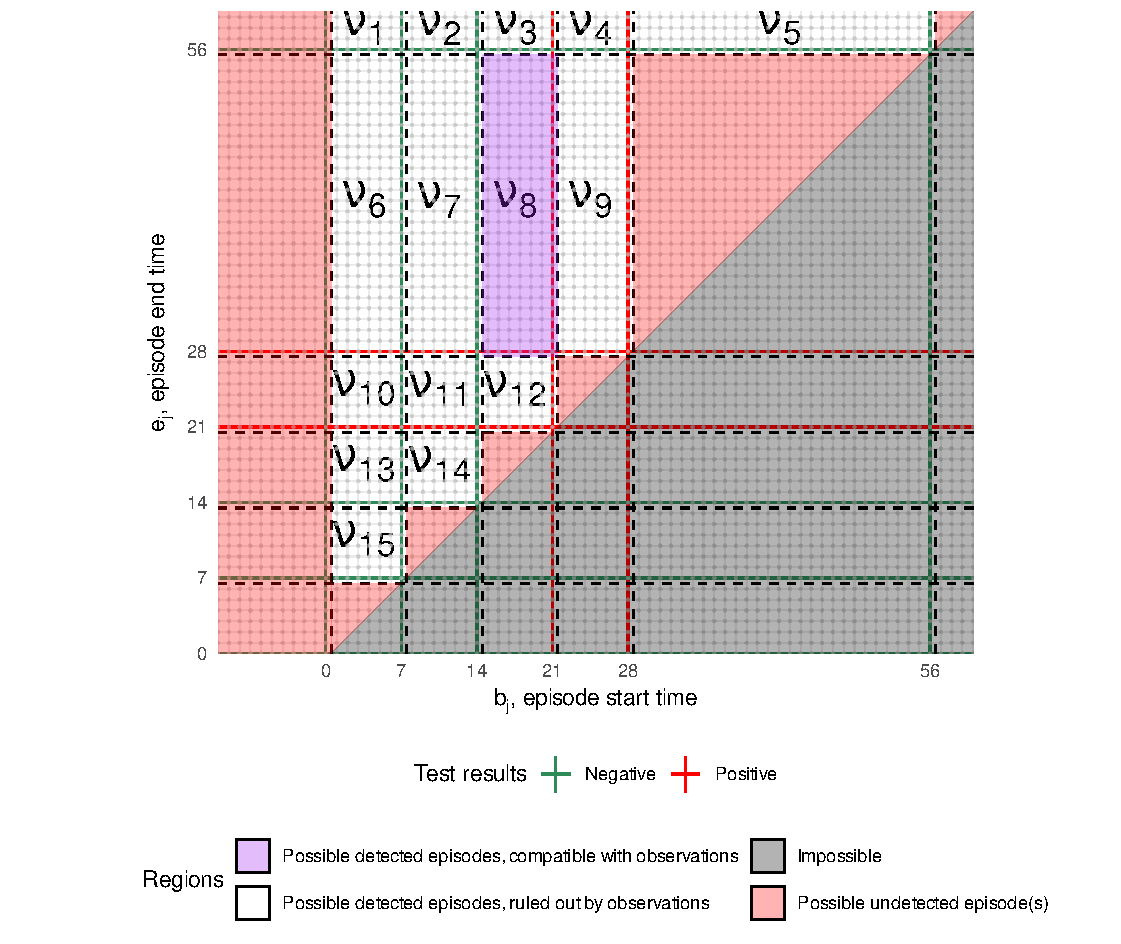
\includegraphics[width=0.9\paperwidth]{figures/output/regions_diag}}
\thisfloatpagestyle{empty}
\caption[Episode regions]{%
  Each dot is a combination of $b_j$ and $e_j$ for an arbitrary individual $i$.
  Each box, bounded by dashed lines, are combinations giving $O(j) = \vec{\nu}_k$, $k$ corresponding to the numeric label; labels are arbitrary but unique across all individuals.
  $i$ had negative tests at times 0, 7, 14, 56, and 84 (not shown) and positive tests at times 21 and 28.
  The purple region corresponds to the doubly interval censored episode in this individual.
  That is, $n_8 = 1$ and $n_k = 0$ for $k = 1, \dots, 7, 9, \dots, 15$.
  The red region corresponds to combinations giving $O(j) = \emptyset$.
  Impossible region violates $b_j \leq e_j$.
}
\label{perf-test:fig:partitionSpace}
\end{figure}

In the CIS data, each $n_k$ ($k \neq u$) is observed as either 0 or 1.
Define $\set{D} = \{ k \ssep n_k = 1 \}$, the detected episodes.
Furthermore, note that the support of the multinomial distribution requires that $\nnodet = \ntot - \ndet$.
Let $\na = [n_{1}, \dots, n_{N_E}]^T$ be the observed portion of $\vec{n}$.
Then \cref{perf-test:eq:multinomial-ll} simplifies to:
\begin{align}
  p(\vec{n} \mid \ntot, \vec{\theta})
  &= p(\na \mid \ntot, \vec{\theta}) \\
  &= \frac{\ntot!}{(\ntot - \ndet)!} p_u^{\ntot-\ndet} \prod_{k \in \set{D}} p_k.
  \label{perf-test:eq:multinomial}
\end{align}

The relevant information from the CIS data is fully contained in the vector $\na$.
Therefore, the posterior of interest is:
\begin{align}
p(\vec{\theta} \mid \na)
&\propto p(\vec{\theta}) p(\na \mid \vec{\theta}) \\
&= p(\vec\theta) \sum_{\ntot= \ndet}^{\infty} p(\ntot, \na \mid \vec{\theta}) \\
&= p(\vec{\theta}) \sum_{\ntot=\ndet}^\infty p(\ntot \mid \vec{\theta}) p(\na \mid \ntot, \vec{\theta}) \\
&= p(\vec{\theta}) \sum_{\ntot=\ndet}^\infty p(\ntot \mid \vec{\theta}) \frac{\ntot!}{(\ntot - \ndet)!} \pnodet^{\ntot - \ndet} \prod_{k \in \set{D}} p_k &\text{by \cref{perf-test:eq:multinomial}} \\
&= p(\vec{\theta}) \left( \prod_{k \in \set{D}} p_k \right) \left( \sum_{\ntot=\ndet}^\infty p(\ntot \mid \vec{\theta}) \frac{\ntot!}{(\ntot - \ndet)!} \pnodet^{\ntot - \ndet} \right).
\label{perf-test:eq:posterior1}
\intertext{For convenience, define the summation term as:}
\eta &= 
\sum_{\ntot=\ndet}^\infty p(\ntot \mid \vec{\theta}) \frac{\ntot!}{(\ntot - \ndet)!} \pnodet^{\ntot - \ndet}.
\label{perf-test:eq:eta}
\end{align}
The rest of this section derives expressions for each of $p_{k}$, $p_{u}$ and $\eta$.

\subsection{Expression for $\eta$}

\todo[inline]{This derivation could be moved to supp material?}

We derive an analytical solution to $\eta$ (defined in \cref{perf-test:eq:eta}).
We assume the prior $\ntot \dist \NBc(\mu, r)$, and that it is independent of $\vec{\theta}$, the parameters of the survival distribution.
Therefore, $p(\ntot \mid \vec{\theta}) = p(\ntot)$.
This assumption makes $\eta$ analytically tractable, allowing computationally feasible inference.

Putting a negative binomial prior on $\ntot$ is equivalent to the following gamma-Poisson composite; its use simplifies the derivation.
\begin{align}
\ntot \mid \lambda &\dist \Poi(\lambda) \\
\lambda &\dist \GamDist(a, b)
\end{align}
where $b = r / \mu$ and $a = r$.
Hence:
\begin{align}
\eta
&= \int \sum_{\ntot=\ndet}^\infty \frac{\ntot!}{(\ntot-\ndet)!} \pnodet^{\ntot-\ndet} p(\ntot \mid \lambda) p(\lambda) d\lambda &\text{$\lambda$ explicit}\\
&= \int \sum_{\ntot=\ndet}^\infty \frac{\ntot!}{(\ntot-\ndet)!} \pnodet^{\ntot-\ndet} \frac{\lambda^{\ntot} e^{-\lambda}}{\ntot!} p(\lambda) d\lambda &\ntot \dist \Poi\\
%&= \int \sum_{\ntot=\ndet}^\infty \frac{1}{(\ntot-\ndet)!} \pnodet^{\ntot-\ndet} \lambda^{\ntot-\ndet} \lambda^{\ndet} e^{-\lambda} p(\lambda) d\lambda \\
&= \int \lambda^{\ndet} e^{-\lambda} p(\lambda) \sum_{\nnodet=0}^\infty \frac{(\pnodet \lambda)^{\nnodet}}{\nnodet!} d\lambda &\nnodet = \ntot-\ndet\\
&= \int \lambda^{\ndet} e^{-\lambda} p(\lambda) e^{\lambda \pnodet} d\lambda &\text{Maclaurin series of $e$} \\
&= \int \lambda^{\ndet} e^{-\lambda(1 - \pnodet)} \frac{b^a}{\Gamma(a)} \lambda^{a-1} e^{-b\lambda} d\lambda &\lambda \dist \GamDist\\
&= \int \frac{b^a}{\Gamma(a)} \lambda^{a+\ndet-1} e^{-(b+1-\pnodet)\lambda} d\lambda \\
&= \frac{b^a}{\Gamma(a)} \frac{\Gamma(a+\ndet)}{(b+1-\pnodet)^{a+\ndet}} &\text{Gamma pdf}\\
&\propto (b+1-\pnodet)^{-(a+\ndet)} &\text{only $p_u$ depends on $\theta$}\\
&= (r/\mu + 1 - \pnodet)^{-(r+\ndet)} &\text{sub in $\mu$ and $r$}\\
&\propto(r + \mu (1- \pnodet))^{-(r+\ndet)}.
\end{align}

Substituting this into \cref{perf-test:eq:posterior1} gives:
\begin{align}
p(\vec{\theta} \mid \na)
&\propto p(\vec{\theta}) \left( \prod_{i \in \set{D}} p_k \right) (r + \mu (1- \pnodet))^{-(r+\ndet)} \label{perf-test:eq:full-posterior}.
\end{align}


\subsection{Deriving $p_k$}

Recall the definitions $p_k = \prob(O(j) = \vec{\nu}_k \mid \vec{\theta})$ where $O(j)$ are the observations of episode $j$ and $\vec{\nu}_k = [l^{(b)}_k, r^{(b)}_k, l^{(e)}_k, r^{(e)}_k, i_k]^T$.

Decompose $p_k$ as $p_k = p_{ik} \prob(i(j) = i_k \mid \vec{\theta})$
where $p_{ik} = \prob(O(j) = \vec{\nu}_k \mid i(j) = i_k, \vec{\theta})$.
% This is valid as $\prob(O(j) = \nu_k \mid i(j) \neq i_k) = 0$ due to the condition here being equivalent to equating the two vectors' final elements.
Assume that each infection episode occurs independently and with equal probability in any individual, \ie $\prob(i(j) = i_k) = 1/\Ncis$ for all $j$ and $k$.

If $i(j) = i_k$ then the event $O(j) = \vec{\nu}_k$ occurs if and only if the episode starts in the interval $[l^{(b)}_k, r^{(b)}_k]$ and ends in the interval $[l^{(e)}_k, r^{(e)}_k]$.
Omitting the conditioning on $\vec{\theta}$ and $i(j) = i$, this gives:
\todo[inline]{this derivation might be too verbose for the main text}
\begin{align}
p_{ik}
=& \prob \left( l_k^{(b)} \leq B_{j} \leq r_k^{(b)}, l_k^{(e)} \leq E_{j} \leq r_k^{(e)} \right) \\
=& \prob \left( l_k^{(e)} \leq E_{j} \leq r_k^{(e)} \mid l_k^{(b)} \leq B_{j} \leq r_k^{(b)} \right) \times\prob \left( l_k^{(b)} \leq B_{j} \leq r_k^{(b)} \right) \\
=& \sum_{b = l_k^{(b)}}^{r_k^{(b)}} \prob \left( l_k^{(e)} \leq E_{j} \leq r_k^{(e)} \mid B_{j} = b \right) \prob \left(B_{j} = b \right) \\
=& \sum_{b = l_k^{(b)}}^{r_k^{(b)}} \prob \left( l_k^{(e)} - b + 1 \leq D_{j} \leq r_k^{(e)} - b + 1 \right) \prob \left(B_{j} = b \right) &\text{by def of $D_{j}$} \\
=& \sum_{b = l_k^{(b)}}^{r_k^{(b)}} \left( S_{\vec{\theta}}(l_k^{(e)} - b + 1) - S_{\vec{\theta}}(r_k^{(e)} - b + 2) \right) \prob \left(B_{j} = b \right) &\text{by def of $S_{\vec{\theta}}$} \\
\propto& \sum_{b = l_k^{(b)}}^{r_k^{(b)}} \left( S_{\vec{\theta}}(l_k^{(e)} - b + 1) - S_{\vec{\theta}}(r_k^{(e)} - b + 2) \right)
\label{perf-test:eq:pia}
\end{align}
under the assumption of uniform probability of infection time.
This is the standard form of the likelihood for doubly interval censored data without truncation~\cite[e.g.][]{sunEmpirical}.

\subsection{Deriving $1 - p_u$} \label{perf-test:sec:prob-undetected}

The final component of \cref{perf-test:eq:full-posterior} required is $1 - p_u$.
Recall the definition $p_u = \prob(O(j) = \emptyset \mid \vec{\theta})$.
Therefore:
\begin{align}
  1 - p_u
  &= 1 - \sum_{i=1}^{\Ncis} \prob(O(j) = \emptyset, i(j) = i \mid \vec{\theta}) \\
  &= 1 - \sum_{i=1}^{\Ncis} \prob(O(j) = \emptyset \mid i(j) = i \mid \vec{\theta}) P(i(j) = i \mid \vec{\theta}) \\
  &= 1 - \frac{1}{\Ncis}\sum_{i=1}^{\Ncis} \prob(O(j) = \emptyset \mid i(j) = i \mid \vec{\theta}) \\
  &= \frac{1}{\Ncis} \sum_{i=1}^{\Ncis} (1 - \prob(O(j) = \emptyset \mid i(j) = i \mid \vec{\theta}))
  \label{perf-test:eq:pu}
\end{align}
assuming $P(i(j) = i \mid \vec{\theta}) = 1/\Ncis$ as before.
Let $p_{iu} = \prob(O(j) = \emptyset \mid i(j) = i, \vec{\theta})$.
Therefore, the crucial component is $1 - p_{iu}$.
This is one minus the probability that an episode in individual $i$ was undetected, \ie the probability of the episode being detected.

An episode $j$ in individual $i(j)$ is detected if and only if all the following conditions are met.
\begin{enumerate}
    \item $\exists t \in \sched_{i(j)}$ such that $b_j \leq t \leq e_j$; this condition is equivalent to having at least one positive test for the episode.
    \item $b_j > \min \sched_{i(j)}$.
      For individuals enrolled during the period considered ($\min \sched_{i(j)} > 0$), this ensures that the beginning of the episode is lower bounded; thereby adjusting for those who enrolled during the period being less likely to have a detected infection.
      For individuals enrolled prior to the period considered ($\min \sched_{i(j)} \leq 0$), this means that the episode was not detected prior to time 1.
    \item $b_j \leq T_{i(j)}$ where $T_{i(j)} = \max \{ t \in \sched_{i(j)} \ssep t \leq T \}$ is the last time that $i(j)$ is tested in the period, meaning that the test is detected within the period.
    \item $\exists t \in \sched_{i(j)}$ such that $t > e_j$, upper bounding the end of the episode.
      For episodes detected in the period we consider, a negligible number of episodes are excluded due to this critera.
      It only occurs in individuals lost to follow-up; therefore, we neglect this possibility.
      % For a new context, including recent infections, this condition could be relaxed by considering episodes that do not meet this criterion as right censored.
\end{enumerate}

% An episode is undetected if and only if no tests are performed during the episode or if there was no negative test prior to the episode.
% Equivalently, that the first test at or after $b$ is after $e$, or that there is no negative test prior to $b$.
First define $\tau_{\sched_i}(t)$ as the time until the next test at or after time $t$ in the schedule $\sched_i$:
\begin{align}
\tau_{\sched_i}(t) &= \min \{ t' \in \sched_i : t' \geq t \} - t
\label{perf-test:eq:tau-def}
\end{align}
% defining $\min \emptyset = \infty$; \ie $\tau_{\sched_i}(t) = \infty$ if there is no $t' \in \sched_i$ such that $t' \geq t$.
The first condition can now be expressed as $e_j \geq b_j + \tau_{\sched_{i(j)}}(b_j)$.
Equivalently, $d_j \geq \tau_{\sched_{i(j)}}(b_j) + 1$.
% The fourth condition can be expressed as $\tau_{\sched_{i(j)}}(b_j) < \infty$.


% Then $\Omega_i$ can be written as:
% \begin{align}
% \Omega_i = \{ (b, e) \ssep \tau_{\sched_i}(b) + b > e \vee b \leq \min(\sched_i) \}.
% \end{align}
Therefore, omitting the conditioning on $\vec{\theta}$ and $i(j) = i$:
\begin{align}
1 - p_{iu}
% &= 1 - \prob((B_{j}, E_{j}) \in \Omega_i) \\
&= \prob(D_j \geq \tau_{\sched_{i}}(B_j)+ 1, \min \sched_{i(j)} < B_j \leq T_{i(j)}) \\
&= \sum_{b = \min \sched_{i} + 1}^{T_{i(j)}} \prob(D_j \geq \tau_{\sched_{i}}(b) + 1 \mid B_j = b) \prob(B_j = b)\\
&\propto \sum_{b = \min \sched_{i} + 1}^{T_{i(j)}} S_{\vec{\theta}}(\tau_{\sched_{i}}(b) + 1).
\label{perf-test:eq:piu}
\end{align}

Substituting into \cref{perf-test:eq:pu}:
\begin{align}
1 - p_u
& \propto \sum_{i=1}^{\Ncis} \sum_{b = \min \sched_{i} + 1}^{T_{i(j)}} S_{\vec{\theta}}(\tau_{\sched_{i}}(b) + 1).
\end{align}

\subsection{False negatives}

Now we modify the survival framework to incorporate false negatives.
We use the model with a constant test sensitivity to ensure the likelihood remains tractable.

\subsubsection{Modifying \texorpdfstring{$p_{ia}$}{pia}} \label{imperf-test:sec:modifying-p_ia}

We will modify $p_{ia}$ to allow the negative test following the last positive to be a false negative.
If it is a false negative, then we will consider the episode's end right-censored.
However, if it is a true negative, then the episode's end is interval censored, as previously.
A mixture of these scenarios forms the episode's likelihood contribution, with the mixture probability determined by the test sensitivity.

We start by finding the tests that need consideration.
For tractability and simplicity, we consider only tests between the negative tests providing an upper bound on the length of the episode.
By definition (see \cref{E-biology-data:sec:cis-episodes}), these are the tests between $l_{j(i)}^{(b)} - 1$ and $r_{j(i)}^{(e)} + 1$ inclusive.
They are a subset of $\sched_i$, the set of test times for the individual in which episode $i$ occurs.

For tractability, assume that the negative test bounding the start of the episode, on day $l_{j(i)}^{(b)}-1$, is a true negative.
This assumption is reasonable because, since a positive test follows at $r_{j(i)}^{(b)}$, the negative at $l_{j(i)}^{(b)}-1$ is likely early in the infection and the test sensitivity is high early in an infection.
Therefore, this is unlikely to be a false negative because, if the individual was detectable at this time, they are in a period with high test sensitivity.
This true negative, occurs with probability 1, and hence does not contribute to the likelihood.
Denote the remaining tests considered as $\sched'_i = \{ t \in \sched_i \ssep r_{j(i)}^{(b)} \leq t \leq r_{j(i)}^{(e)} + 1 \}$, and their results by $\vec{y_{j(i)}} = \{ y_{j(i)}(t) \ssep t \in \sched'_i \}$ where $y_{j(i)}(t) = 1$ if the test on day $t$ is positive and 0 otherwise.

As we assume that there are no false positives, the infection episode must span at least the period $[r^{(b)}_{j(i)}, l^{(e)}_{j(i)}]$ because it starts and ends with a positive test.
This includes all $t \in \sched'_i$ except $t = r_{j(i)}^{(e)}+1$.
Therefore, the test results at times in $\sched_i'$, except the test at $r_{j(i)}^{(e)}+1$, are either true positives or false negatives.

Consider the negative test at $r_{j(i)}^{(e)}+1$, the first negative after the start of the episode which may be a false negative.
It is a false negative if and only if the episode ends after the test, \ie $e_{j(i)} > r_{j(i)}^{(e)}$.
We proceed by considering whether this is the case, and considering the case with $b_{j(i)}$ known; $b_{j(i)}$ will later be integrated out.

First, if $e_{j(i)} \leq r_{j(i)}^{(e)}$, meaning that the test at $r_{j(i)}^{(e)}+1$ is a true negative and the end of the episode is interval censored as in the previous chapter.
% In this case, the test at $r_{j(i)}^{(e)} + 1$ is a true negative, as are all other tests not in $\sched'_i$.
The true negative occurs with probability 1, by the assumption of no false positives.
\begin{align}
&p(\vec{y_{j(i)}}, e_{j(i)} \leq r_{j(i)}^{(e)} | b_{j(i)}, p_\text{sens}, \theta) \\
&= p(\vec{y_{j(i)}}, l_{j(i)}^{(e)} \leq e_{j(i)} \leq r_{j(i)}^{(e)} | t_i, b_{j(i)}, p_\text{sens}, \theta) \\ % &\text{as no false positives}
&= p(\vec{y_{j(i)}} \mid l_{j(i)}^{(e)} \leq e_{j(i)} \leq r_{j(i)}^{(e)}, t_i, b_{j(i)}, p_\text{sens}, \theta) p(l_{j(i)}^{(e)} \leq e_{j(i)} \leq r_{j(i)}^{(e)} | t_i, b_{j(i)}, p_\text{sens}, \theta) \\
&= \left( \prod_{t \in \sched'_i} p_\text{sens}^{y_{j(i)}(t)} (1 - p_\text{sens})^{(1 - y_{j(i)}(t))} \right) \left( S_\theta(l_{j(i)}^{(e)} - b_{j(i)} - 1) - S_\theta(r_{j(i)}^{(e)} - b_{j(i)} - 1) \right)
\label{imperf-test:eq:ll-ei-lt-ri}
\end{align}

Second, if $e_{j(i)} > r_{j(i)}^{(e)}$.
In this case, the test at $r_{j(i)}^{(e)}$ is a false negative, occurring with probability $(1 - p_\text{sens})$.
To avoid having to consider tests after $r_{j(i)}^{(e)}$, which could greatly complicate the likelihood, I model this case as the episode being right-censored at $r_{j(i)}^{(e)}$.
Taking the same approach as before:
\begin{align}
&p(\vec{y_{j(i)}}, e_{j(i)} > r_{j(i)}^{(e)} | b_{j(i)}, p_\text{sens}, \theta) \\
&= p(\vec{y_{j(i)}} \mid e_{j(i)} > r_{j(i)}^{(e)}, t_i, b_{j(i)}, p_\text{sens}, \theta) p(e_{j(i)} > r_{j(i)}^{(e)} | t_i, b_{j(i)}, p_\text{sens}, \theta) \\
&= \left( \prod_{t \in \sched'_i} p_\text{sens}^{y_{j(i)}(t)} (1 - p_\text{sens})^{(1 - y_{j(i)}(t))} \right) (1 - p_\text{sens}) S_\theta(r_{j(i)}^{(e)} - b_{j(i)} - 1)
\label{imperf-test:eq:ll-ei-gt-ri}
\end{align}

These expressions can now be used to form the full replacement for $p_{ia}$, $p'_{ia}$, the likelihood of the data $\vec{y_{j(i)}}$.
First, augment the data with $b_{j(i)}$, and split into the cases just discussed:
\begin{align}
p_{ia}'
&= p(\vec{y_{j(i)}} \mid p_\text{sens}, \theta) \\
&= \sum_{b_{j(i)} = l_{j(i)}^{(b)}}^{r_{j(i)}^{(b)}} \left( p(\vec{y_{j(i)}}, e_{j(i)} \leq r_{j(i)}^{(e)} \mid b_{j(i)}, p_\text{sens}, \theta) + p(\vec{y_{j(i)}}, e_{j(i)} > r_{j(i)}^{(e)} \mid b_{j(i)}, p_\text{sens}, \theta) \right) p(b_{j(i)} \mid p_\text{sens}, \theta).
\intertext{Now, substitute in \cref{imperf-test:eq:ll-ei-lt-ri,imperf-test:eq:ll-ei-gt-ri}, then take out the common factor:}
&= \left( \prod_{t \in \sched'_i} p_\text{sens}^{y_{j(i)}(t)} (1 - p_\text{sens})^{(1 - y_{j(i)}(t))} \right) \\ & \ \times \sum_{b_{j(i)} = l_{j(i)}^{(b)}}^{r_{j(i)}^{(b)}} \left( S_\theta(l_{j(i)}^{(e)} - b_{j(i)} - 1) - S_\theta(r_{j(i)}^{(e)} - b_{j(i)} - 1) + (1 - p_\text{sens}) S_\theta(r_{j(i)}^{(e)} - b_{j(i)} - 1) \right) \\ & \ \times p(b_{j(i)} \mid p_\text{sens}, \theta) \\
&= \left( \prod_{t \in \sched'_i} p_\text{sens}^{y_{j(i)}(t)} (1 - p_\text{sens})^{(1 - y_{j(i)}(t))} \right) \\ & \ \times \sum_{b_{j(i)} = l_{j(i)}^{(b)}}^{r_{j(i)}^{(b)}} \left( S_\theta(l_{j(i)}^{(e)} - b_{j(i)} - 1) - p_\text{sens} S_\theta(r_{j(i)}^{(e)} - b_{j(i)} - 1) \right) p(b_{j(i)} \mid p_\text{sens}, \theta).
\label{imperf-test:eq:pia-prime}
\end{align}
Note that if $p_\text{sens} = 1$ then $p_{ia}' = p_{ia}$.

If $\psens$ is fixed (\ie has a point prior) and $p(b_{j(i)} \mid \psens, \theta) \propto 1$ (as assumed in \cref{E-perf-test}) then:
\begin{align}
p_{ia}'
&\propto \sum_{b_{j(i)} = l_{j(i)}^{(b)}}^{r_{j(i)}^{(b)}} S_\theta(l_{j(i)}^{(e)} - b_{j(i)} - 1) - p_\text{sens} S_\theta(r_{j(i)}^{(e)} - b_{j(i)} - 1).
\label{imperf-test:eq:pia-prime-constant}
\end{align}

\subsubsection{Modifying \texorpdfstring{$p_{iu}$}{piu}} \label{imperf-test:sec:modifying-p_iu}

Several mechanisms for episodes being undetected were considered when deriving $p_{iu}$ in \cref{perf-test:eq:piu}.
We now consider the additional mechanisms arising due to false negatives.
Specifically, episode $i$ could be undetected if the first test after the $b_{j(i)}$, episode $i$'s start day, is a false negative and then there are no subsequent positive tests.

This false negative would occur at the first test after the infection episode begins, on day $b_{j(i)} + \tau_{\sched_i}(b_{j(i)})$ (see \cref{E-perf-test:sec:model}).
A false negative occurring requires that the episode has not yet ended but a negative still occurs.
The episode has not yet ended at the time of the test if $e_{j(i)} = b_{j(i)} + d_i - 1$ is after the test, that is the duration of the infection $d_i > \tau_{\sched_i}(b_{j(i)})$.
Conditional on the episode having not yet ended, the test result is negative with probability $1 - \psens$.

For there to be no subsequent positive tests, all tests up until day $e_{j(i)}$ are false negatives.
We assume there is a negligible probability of two false negatives.
Therefore, this can only occur if the episode ends before another test.
Denote the number of days between $b_{j(i)}$ and the test following the false negative as $\tau^2_{\sched_i}(b_{j(i)}) \stackrel{\text{def}}{=} \tau_{\sched_i}(\tau_{\sched_i}(b_{j(i)}) + 1)$.
Then, the episode ends before this test if $d_i < \tau^2_{\sched_i}(b_{j(i)})$.

Therefore, this mechanism causes episode $i$ to be undetected if all the following conditions hold.
\begin{enumerate}
    \item The episode would have been detected considering only the mechanisms in \cref{perf-test:eq:piu}. That is $b_{j(i)} > \min(\sched_i)$ and $\tau_{\sched_i}(b_{j(i)}) + b_{j(i)} \leq e_{j(i)}$.
    \item The episode ends in the interval $[\tau_{\sched_i}(b_{j(i)}) + b_{j(i)}, \tau^2_{\sched_i}(b_{j(i)}) + b_{j(i)}]$.
      Note that the lower bound here is exactly the bound on $e_{j(i)}$ in the previous condition.
      Equivalently, $\tau_{\sched_i}(b_{j(i)}) + 1 \leq d_i \leq \tau^2_{\sched_i}(b_{j(i)}) + 1$.
    \item A false negative occurs on day $\tau_{\sched_i}(b_{j(i)}) + b_{j(i)}$. Conditional on the previous condition, this occurs with probability $1 - \psens$.
\end{enumerate}

The probability of this occurring, conditional on $B_{j(i)} = b_{j(i)} > \min(\sched_i)$ is:
\begin{align}
&\prob \left(
    \tau_{\sched_i}(b_{j(i)}) + 1 \leq D_i \leq \tau^2_{\sched_i}(b_{j(i)}) + 1
    \mid b_{j(i)},
\theta \right) (1 - \psens) \\
&= \left( S_\theta(\tau_{\sched_i}(b_{j(i)}) + 1) - S_\theta(\tau^2_{\sched_i}(b_{j(i)}) + 1) \right) (1 - \psens).
\end{align}
Integrating over $b_{j(i)}$ for $\min \sched_i < b_{j(i)} \leq T$ ($T$ being the last day of the period considered), in the same way as \cref{perf-test:eq:piu}, gives:
\begin{align}
\eta = (1 - p_\text{sens})\frac{1}{T} \sum_{b=\min(\sched_i) + 1}^T \left( S_\theta(\tau_{\sched_i}(b) + 1) - S_\theta(\tau^2_{\sched_i}(b) + 1) \right).
\end{align}

Denote the replacement for $p_{iu}$ as $p_{iu}'$.
$p_{iu}'$ is the probability of episode $i$ being missed, considering both the mechanisms from \cref{E-perf-test} and the new mechanism here.
These mechanisms are mutually exclusive.
Hence, $p_{iu}'$ is the sum of these, $p_{iu}' = p_{iu} + \eta$.
For the posterior density, \cref{E-perf-test:eq:full-posterior}, $1 - p_{iu}'$ is the required quantity.
\begin{align}
1 - p_{iu}'
&= 1 - p_{iu} - (1 - p_\text{sens})\frac{1}{T} \sum_{b=\min(\sched_i) + 1}^T \left( S_\theta(\tau_{\sched_i}(b) + 1) - S_\theta(\tau^2_{\sched_i}(b) + 1) \right) \\
&= \frac{1}{T} \sum_{b=\min(\sched_i) + 1}^T \left( p_\text{sens} S_\theta(\tau_{\sched_i}(b) + 1) + (1 - p_\text{sens}) S_\theta(\tau^2_{\sched_i}(b) + 1)\right).
\label{imperf-test:eq:pit-prime}
\end{align}

$p_{iu}'$ and $p_{ia}'$ are substituted for $p_{iu}$ and $p_{ia}$ respectively in \cref{E-perf-test:eq:full-posterior}.
The posterior density is otherwise unchanged.



\subsection{Incorporating prior information}

\todo[inline]{A bunch of this can probably be cut / moved to supp material. Supp material should also contain the ATACCC analysis.}

The information from \cref{E-ATACCC} can be incorporated through the prior.
This is desirable because the ATACCC study frequently sampled individuals early in the infection.
Therefore, \cref{E-ATACCC}'s estimate of the survival distribution in the early infection period should be reliable.
In the later infection period, the ATACCC study has fewer observations and hence the estimates are less reliable.
CIS can inform the posterior in this region.

When constructing the prior, two aspects need consideration.
Firstly, the model structure from \cref{E-ATACCC} leads to positive correlation in the posterior estimates of the hazard, which should be propagated into this analysis.
That is, the prior used in this analysis cannot be independent across the hazards.
Secondly, the uncertainty in the estimates from \cref{E-ATACCC} should be increased for this analysis.
The additional uncertainty is because the \cref{E-ATACCC} analysis extrapolates beyond the data using strong model assumptions (see \cref{E-ATACCC:sec:discussion}).
%Furthermore, there are differences in the study design and laboratories used between the two studies (see \cref{E-intro:sec:studies}) which may mean that results do not generalise between the studies.
We form the prior for the combination in two steps.

We first approximate the \cref{E-ATACCC} posterior estimate of the hazard as a multivariate normal on the logit scale.
This can be viewed as an approximation of Markov melding~\cite{goudieJoining}.
Using a multivariate normal, as opposed to multiple univariate distribution, ensures that the correlation between the hazards is preserved.
The logit transformation maps from the $[0, 1]$ interval to the full real line.
To estimate the parameters of the multivariate normal, we use the method of moments.
The approximation is very good (see \cref{perf-test:fig:approximate-ATACCC-hazard} and \cref{perf-test:fig:approximate-ATACCC-survival}).
\begin{figure}
  \thisfloatpagestyle{empty}
  \vspace{-2.5cm}
%   \makebox[\textwidth][c]{\includegraphics[width=.9\paperwidth]{cis-perfect-testing/ataccc-approximation-hazard}}
  \caption[Approximating the ATACCC posterior hazard as a logit-normal]{Comparison of the posterior estimate of the hazard from \cref{E-ATACCC} and its approximation with a logit-normal distribution (kernel density estimate smoothed) for the first 15 hazards. \label{perf-test:fig:approximate-ATACCC-hazard}}
\end{figure}
\begin{figure}
%   \centering \includegraphics{cis-perfect-testing/ataccc-approximation-survival}
  \caption[Approximating the ATACCC posterior survival as a logit-normal]{Comparison of the posterior estimate of the survival from \cref{E-ATACCC} and its approximation with a logit-normal distribution (median and central 95\% interval). The survival is a function of all the hazards up until that point, therefore the correlation between the hazards must be well-approximated to have these agree. \label{perf-test:fig:approximate-ATACCC-survival}}
\end{figure}

Having approximated the estimate as a multivariate normal, I add additional uncertainty using a discrete Beta process.
The discrete Beta process prior generalises the form of prior used in \cref{perf-test:sec:independent-priors} by allowing the central estimate of the hazard to vary over time~\cite{ibrahimBayesian,sunStatisticala}.
It is:
\begin{align}
  \lambda_t &\sim \text{Beta}(\alpha_t, \beta_t) &t = 1, 2, \dots \\
  \alpha_t &= k_t h_t + \alpha_0 \\
  \beta_t &= k_t (1 - h_t) + \beta_0
\end{align}
where $k_t$, $\alpha_0$, and $\beta_0$ are hyperparameters; and $h_t$ is a point estimate of the hazard at time $t$ from ATACCC.
An intuition for what this distribution represents can be gained from a conjugate model for $\lambda_t$ with a beta prior and a binomial likelihood.
If $\lambda_t$ is given the prior distribution $\text{Beta}(\alpha_0, \beta_0)$, and we then have $k_t$ observations with $k_t h_t$ successes, then the posterior distribution for $\lambda_t$ is $\text{Beta}(\alpha_t, \beta_t)$ (as defined above).

$k_t$ reflects the subjective belief that the estimates from \cref{E-ATACCC} are very reliable in the early infection period but unreliable by day 30.
The equation for $k_t$ is below and shown in \cref{perf-test:fig:kt}.
\begin{align}
k_t = \begin{cases}
  \expit(-0.4 * (t - 20)) &\text{for $t \leq 39$} \\
  0 &t > 39
\end{cases}
\end{align}
where $\expit(x) = 1 / (1 + \exp(-x))$.

\begin{figure}
%   \centering \includegraphics{cis-perfect-testing/kt-prior}
  \caption{Function used for $k_t$. \label{perf-test:fig:kt}}
\end{figure}

\section{Simulation study}

\section{Application to real study data}

\section{Discussion}

\bigskip
\begin{center}
{\large\bf SUPPLEMENTARY MATERIAL}
\end{center}

\begin{description}

\item[Title:] Brief description. (file type)

\item[R-package for  MYNEW routine:] R-package MYNEW containing code to perform the diagnostic methods described in the article. The package also contains all datasets used as examples in the article. (GNU zipped tar file)

\item[HIV data set:] Data set used in the illustration of MYNEW method in Section~ 3.2. (.txt file)

\end{description}

\section{BibTeX}

We hope you've chosen to use BibTeX!\ If you have, please feel free to use the package natbib with any bibliography style you're comfortable with. The .bst file agsm has been included here for your convenience. 


\bibliographystyle{agsm}

\bibliography{references}
\end{document}
